\chapter{Introduction}

The Traveling Salesman Problem (TSP) stands as an iconic challenge in the field of combinatorial optimization, captivating researchers for its practical significance and theoretical complexity. Originating in the early 20th century, the TSP involves determining the most efficient route for a salesman to visit a set of cities exactly once before returning to the starting point. Despite its seemingly straightforward premise, the exponential growth in potential routes as cities increase presents a formidable computational challenge.

\begin{figure}[htbp]
	\centering
	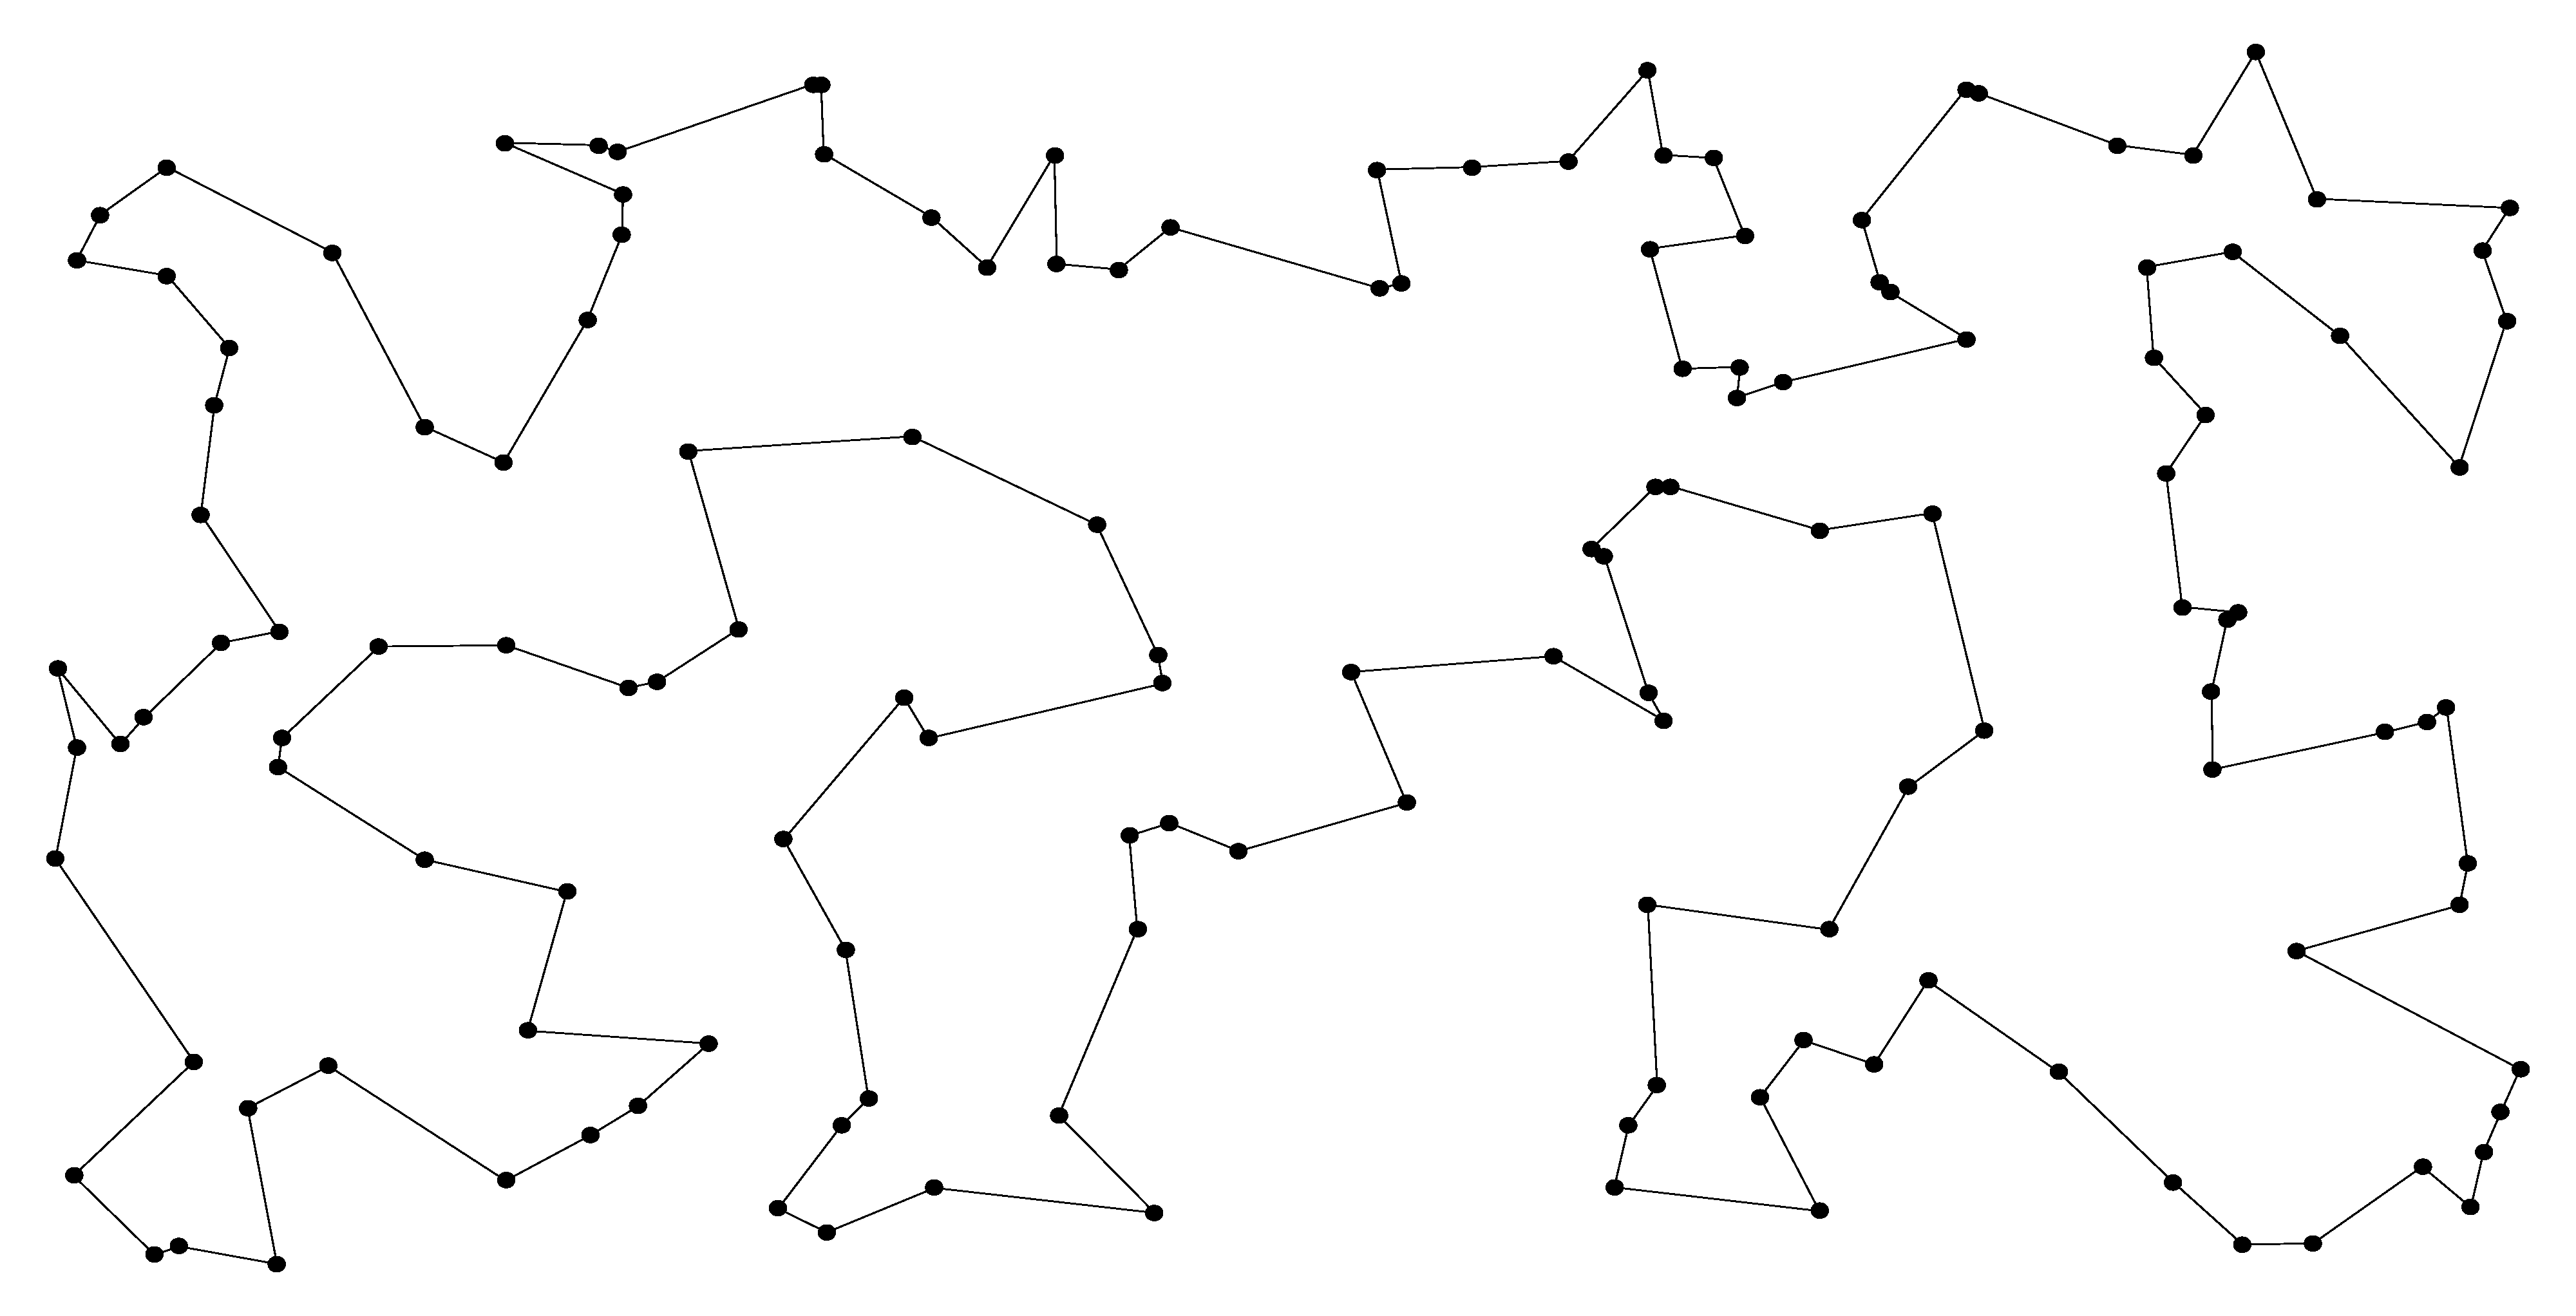
\includegraphics[scale=0.15]{tsp_example}
	\caption{A solution of instance kroA150}
\end{figure}

\section{Complexity of TSP}

The Traveling Salesman Problem (TSP) is renowned not only for its practical applications but also for its classification as an NP-hard problem, signifying its computational complexity and the absence of an efficient algorithm that guarantees an optimal solution within a reasonable timeframe.

This classification as an NP-hard problem implies that as the number of cities to be visited increases, the computation required to find the optimal route escalates exponentially. The TSP's intricate nature lies in its combinatorial explosion: with n cities, the number of possible routes to consider is $(n-1)!/2$, making exhaustive exploration unfeasible for large instances. This exponential growth propels the problem into the realm of computational intractability, where conventional computing methods struggle to provide optimal solutions in a reasonable time frame.

Efforts to solve the TSP have focused on devising algorithms that offer approximate solutions or heuristics that navigate the expansive solution space more efficiently. While exact algorithms exist, such as branch-and-bound techniques, their scalability diminishes as the problem size increases. Heuristic approaches, on the other hand, aim to find near-optimal solutions within acceptable time frames by sacrificing guaranteed optimality for computational tractability.

